\documentclass[a4paper, 12pt, titlepage]{report}
\usepackage{minted}
\usepackage[dvipsnames]{xcolor}
\colorlet{LightApricot}{Orchid!20}
\usepackage{graphicx}
\usepackage{fullpage}
\usepackage{float}
\usepackage{hyperref}
%\usepackage{longtable}
%\usepackage{amsmath}
%\usepackage[normalem]{ulem}
\usepackage{booktabs}
\usepackage{dirtree}
\usepackage{hologo}
\usepackage{csquotes}
\usepackage{tikz}
\usetikzlibrary{shapes.geometric, arrows}

%\usepackage{array}
%\usepackage{tikz}
%\usepackage{parskip}
%\newcommand{\tabitem}{~~\llap{\textbullet}~~}
\setlength{\tabcolsep}{18pt}
\renewcommand{\arraystretch}{1.5}
\renewcommand{\chaptername}{Section}
\hypersetup{
    colorlinks=true,
    linkcolor=blue,
    filecolor=magenta,
    urlcolor=RoyalBlue,
}
\begin{document}
\tikzstyle{startstop} = [rectangle, rounded corners, minimum width=3cm, minimum height=1cm,text centered, draw=black, fill=red!30]
\tikzstyle{io} = [trapezium, trapezium left angle=70, trapezium right angle=110, minimum width=3cm, minimum height=1cm, text centered, draw=black, fill=blue!30]
\tikzstyle{process} = [rectangle, minimum width=3cm, minimum height=1cm, text centered, draw=black, fill=orange!30]
\tikzstyle{decision} = [diamond, minimum width=3cm, minimum height=1cm, text centered, draw=black, fill=green!30]
\tikzstyle{arrow} = [thick,->,>=stealth]
\linespread{1.25}
\author{Affaan Muhammad - 33016763\\Joshua Esterhuizen - 30285976}
\title{ITRI615 - Computer Security\\Project Documentation}
\date{}
\maketitle
\tableofcontents{}

\chapter{Installation and setup}
\section{Project files}
The project files can be found on the following GitHub link:\\
\url{https://github.com/AM-ops/SecurityProject}
\\\\This was our main code repository. We both have been updating the code as we went along and added details and bug fixes to the project.\\\\
To copy the code to your own machine, follow the following steps:
\begin{enumerate}
\item Make sure Git is installed. If not it can be downloaded from here:\\
\url{https://git-scm.com/}
\item Create an empty directory where the code can be copied to
\item Run the following command:
\begin{minted}
[
frame=lines,
framesep=2mm,
baselinestretch=1.2,
bgcolor=LightApricot,
fontsize=\footnotesize,
]
{Shell}
git clone https://github.com/AM-ops/SecurityProject.git
\end{minted}
\end{enumerate}
\section{Virtual Environment}
There are multiple advantages of using virtual environments when creating software. The primary reason being we create a layer of separation and abstraction between our host machine's files and our software project.\\\\
We made use of a Python virtual environment which was handled by Anaconda. This can be downloaded from the following link:\\
\url{https://www.anaconda.com/products/individual}
\subsection{Creating a virtual environment}
Once Anaconda was installed the following commands were run in the terminal to create a virtual environment called \texttt{myDjangoEnv}.
\begin{minted}
[
frame=lines,
framesep=2mm,
baselinestretch=1.2,
bgcolor=LightApricot,
fontsize=\footnotesize,
]
{Shell}
conda create --name myDjangoEnv
\end{minted}
Depending on the version of Anaconda installed you might have to use a leading underscore on Windows machines. The same will apply for commands further down. Below is a demonstration.
\begin{minted}
[
frame=lines,
framesep=2mm,
baselinestretch=1.2,
bgcolor=LightApricot,
fontsize=\footnotesize,
]
{Shell}
_conda create --name myDjangoEnv
\end{minted}
\subsection{Listing virtual environments}
To list all virtual environments on your host machine run the following command.
\begin{minted}
[
frame=lines,
framesep=2mm,
baselinestretch=1.2,
bgcolor=LightApricot,
fontsize=\footnotesize,
]
{Shell}
conda info --envs
\end{minted}
or
\begin{minted}
[
frame=lines,
framesep=2mm,
baselinestretch=1.2,
bgcolor=LightApricot,
fontsize=\footnotesize,
]
{Shell}
conda env list
\end{minted}
\subsection{Deleting a virtual environment}
To delete a virtual environment run the following commands.
\begin{minted}
[
frame=lines,
framesep=2mm,
baselinestretch=1.2,
bgcolor=LightApricot,
fontsize=\footnotesize,
]
{Shell}
conda remove --name <name_of_virtual_environment> --all
\end{minted}
or
\begin{minted}
[
frame=lines,
framesep=2mm,
baselinestretch=1.2,
bgcolor=LightApricot,
fontsize=\footnotesize,
]
{Shell}
conda env remove --name <name_of_virtual_environment>
\end{minted}
\subsection{Activating and deactivating virtual environments}
To activate an environment run the following commands for Windows.
\begin{minted}
[
frame=lines,
framesep=2mm,
baselinestretch=1.2,
bgcolor=LightApricot,
fontsize=\footnotesize,
]
{Shell}
conda activate <name_of_virtual_environment>
\end{minted}
For Linux and MacOS the command is as follows.
\begin{minted}
[
frame=lines,
framesep=2mm,
baselinestretch=1.2,
bgcolor=LightApricot,
fontsize=\footnotesize,
]
{Shell}
source activate <name_of_virtual_environment>
\end{minted}
Once the environment is activated your terminal should change. By default, the active environment, is shown in parentheses () or brackets [] at the beginning of your command prompt as shown below.
\begin{minted}
[
frame=lines,
framesep=2mm,
baselinestretch=1.2,
bgcolor=LightApricot,
fontsize=\footnotesize,
]
{Shell}
(<name_of_virtual_environment>) >_
\end{minted}
Depending on your version of Anaconda to deactivate your environment the commands for Windows is.
\begin{minted}
[
frame=lines,
framesep=2mm,
baselinestretch=1.2,
bgcolor=LightApricot,
fontsize=\footnotesize,
]
{Shell}
deactivate
\end{minted}
or
\begin{minted}
[
frame=lines,
framesep=2mm,
baselinestretch=1.2,
bgcolor=LightApricot,
fontsize=\footnotesize,
]
{Shell}
conda deactivate
\end{minted}
For Linux and MacOS the command will be
\begin{minted}
[
frame=lines,
framesep=2mm,
baselinestretch=1.2,
bgcolor=LightApricot,
fontsize=\footnotesize,
]
{Shell}
source deactivate
\end{minted}
\subsection{Listing Packages installed}
To list all the packages you have installed in an environment there are two methods of listing them.
First, if the environment is not activated run the following.
\begin{minted}
[
frame=lines,
framesep=2mm,
baselinestretch=1.2,
bgcolor=LightApricot,
fontsize=\footnotesize,
]
{Shell}
conda list -n <name_of_virtual_environment>
\end{minted}
Secondly, if the environment is activated, then simply run the following.
\begin{minted}
[
frame=lines,
framesep=2mm,
baselinestretch=1.2,
bgcolor=LightApricot,
fontsize=\footnotesize,
]
{Shell}
conda list
\end{minted}
\subsection{Using pip}
Due to the fact that Python is being used for the project it is always necessary to make sure \texttt{pip} is installed and functioning. If it is not then run the following commands.
\begin{minted}
[
frame=lines,
framesep=2mm,
baselinestretch=1.2,
bgcolor=LightApricot,
fontsize=\footnotesize,
]
{Shell}
conda install -n <name_of_virtual_environment> pip
\end{minted}
\section{Frameworks and other packages}
\subsection{Django}\label{dj}
The primary framework used for development in this project was \texttt{Django}. This is a python based Web framework. The documentation for it can be found here:\\
\url{https://docs.djangoproject.com/en/3.2/}
\subsection{Bootstrap}\label{bs}
Bootstrap is Cascading Style Sheets (CSS) Framework which allows for simple, elegant, and responsive Graphical User Interfaces to be developed for the Web. The documentation for it can be found here:\\
\url{https://getbootstrap.com/docs/5.0/getting-started/introduction/}\\\\
For a more seamless integration of Bootstrap with the \texttt{Django} Framework an additional package called \texttt{django-crispy-forms} was also installed. Its documentation ca be found here:\\
\url{https://django-crispy-forms.readthedocs.io/en/latest/}
\subsection{Miscellaneous}
For typesetting of this documentation, \hologo{LaTeX} was utilised. Additionally, a \hologo{LaTeX} package called \texttt{minted} was used to typeset code in this documentation. Its homepage is located at: \url{https://www.ctan.org/pkg/minted}\\\\
To typeset directory structures in a tree-like manner the \hologo{LaTeX} package \texttt{dirtree} was used. Its homepage can be found at: \url{https://ctan.org/pkg/dirtree}\\\\
To typeset quotations for the Reflection section the \hologo{LaTeX} package \texttt{csquotes} was used. Its homepage can bee found at: \url{https://ctan.org/pkg/csquotes?lang=en}\\\\
Lastly, to typeset code within the HTML pages of our project the JavaScript library called \texttt{Rainbow} was implemented. The GitHub link for that is located at:\\
\url{https://github.com/ccampbell/rainbow}
\chapter{Programming of artefact}
\section{Development Tools}
\subsection{Operating Systems}
The primary systems on which development was done was Linux and Windows 10. The same systems where utilised for testing and bug fixing purposes.
\subsection{IDEs}
For the purposing of coding the following two Integrated Development Environments were used:
\begin{enumerate}
\item Atom. It can be downloaded from: \url{https://atom.io/}
\item Visual Studio Code, also known as VSCode. It can be downloaded from here: \url{https://code.visualstudio.com/}
\end{enumerate}
\subsection{Database Management Tools}
For the purposes of database management, TablePlus was the main software we utilised. It was used to see if our \texttt{Django} models and cryptographic schemes were correctly implemented. TablePlus can be downloaded from: \url{https://tableplus.com/}
\subsection{Hosting}
Due to a number of constraints we landed up running our project locally. The server was \texttt{localhost} and the port number was \texttt{8000}. Therefore the link where we ran our project was:
\url{http://127.0.0.1:8000}
\section{Prerequisites}
\subsection{Project and Package Initialisation}
\textsl{From here on we will refer to the working directory as the directory where the} \texttt{manage.py} \textsl{file is located. This file is created when the project is setup}\\\\
Before our \texttt{Django} project can be created we have to install all the packages mentioned above in Section \ref{dj} and \ref{bs}. A text file called \texttt{requirements.txt} was created which lists the 3 packages we need to install as shown below:
\begin{minted}
[
frame=lines,
framesep=2mm,
baselinestretch=1.2,
bgcolor=LightApricot,
fontsize=\footnotesize,
]
{Text}
django
django-crispy-forms
bootstrap4
\end{minted}
Thereafter the following command was run in the working directory.
\begin{minted}
[
frame=lines,
framesep=2mm,
baselinestretch=1.2,
bgcolor=LightApricot,
fontsize=\footnotesize,
]
{Shell}
pip install -r requirements.txt
\end{minted}
To start a \texttt{Django} project called \texttt{SecProj} the following command was run:
\begin{minted}
[
frame=lines,
framesep=2mm,
baselinestretch=1.2,
bgcolor=LightApricot,
fontsize=\footnotesize,
]
{Shell}
django-admin startproject SecProj
\end{minted}
Your directory should look like the following:
\dirtree{%
.1 /.
.2 manage.py.
.2 SecProj.
.3 \_\_init\_\_.py.
.3 settings.py.
.3 urls.py.
.3 asgi.py.
.3 wsgi.py.
}
\phantom{a}\\
\noindent To verify that your \texttt{Django} project is working run the following command in your working directory:
\begin{minted}
[
frame=lines,
framesep=2mm,
baselinestretch=1.2,
bgcolor=LightApricot,
fontsize=\footnotesize,
]
{Shell}
python manage.py runserver
\end{minted}
You should see the following if you open the link: \url{http://127.0.0.1:8000}
\begin{figure}[H]
\centering
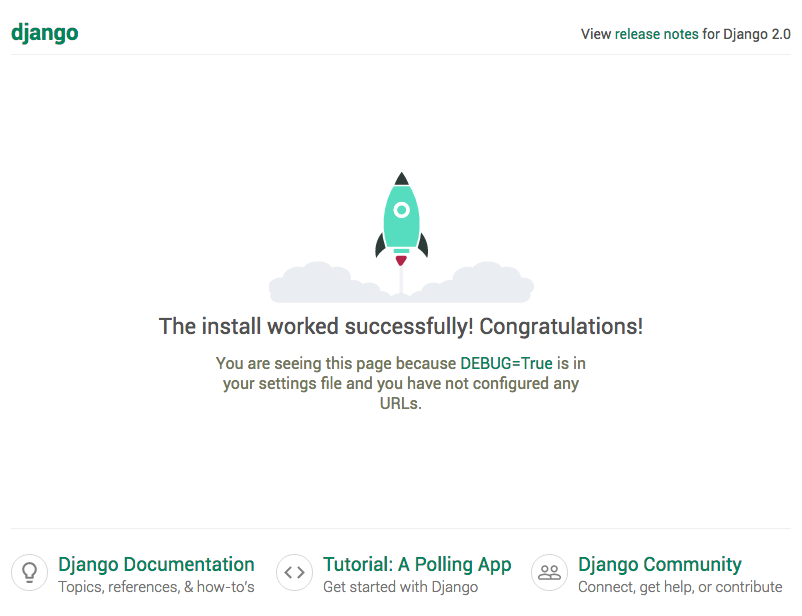
\includegraphics[scale=0.3]{./pics/home}
\caption{Default Homepage of a new Django Project}
\end{figure}
\noindent Now that your \texttt{Django} project is up and running it is time to create a \texttt{Django} 'App' within this project. This App is where we implemented our cryptographic schemes and the bulk of our project. We called our App \texttt{SecApp} and the command to run in your working directory is as follows:
\begin{minted}
[
frame=lines,
framesep=2mm,
baselinestretch=1.2,
bgcolor=LightApricot,
fontsize=\footnotesize,
]
{Shell}
python manage.py startapp SecApp
\end{minted}
Your directory should now look like the following:
\dirtree{%
.1 /.
.2 manage.py.
.2 SecProj.
.3 \_\_init\_\_.py.
.3 settings.py.
.3 urls.py.
.3 asgi.py.
.3 wsgi.py.
.2 SecApp.
.3 \_\_init\_\_.py.
.3 admin.py.
.3 apps.py.
.3 migrations.
.4 \_\_init\_\_.py.
.3 models.py.
.3 tests.py.
.3 views.py.
}
\subsection{Settings and Admin}
The following changes were added to the \texttt{settings.py} file. The whole file is not shown below.
\begin{minted}
[
frame=lines,
framesep=2mm,
baselinestretch=1.2,
bgcolor=LightApricot,
fontsize=\footnotesize,
linenos,
breaklines,
]
{Python}
from pathlib import Path
import os

# Build paths inside the project like this: BASE_DIR / 'subdir'.
BASE_DIR = Path(__file__).resolve().parent.parent
TEMPLATE_DIR = os.path.join(BASE_DIR, 'templates')

# Application definition

INSTALLED_APPS = [
    'django.contrib.staticfiles',
    'bootstrap4',
    'SecProj',
    'SecApp',
    'accounts',
    'crispy_forms',
]
CRISPY_TEMPLATE_PACK = 'bootstrap4'

ROOT_URLCONF = 'SecProj.urls'
TEMPLATES = [{'DIRS': [TEMPLATE_DIR]}]

# Static files (CSS, JavaScript, Images)
# https://docs.djangoproject.com/en/3.1/howto/static-files/

STATIC_URL = '/static/'
STATICFILES_DIR = [os.path.join(BASE_DIR,'static')]
STATICFILES_DIRS = [
    os.path.join(BASE_DIR, "static"),
]
LOGIN_REDIRECT_URL = 'success'
LOGOUT_REDIRECT_URL = 'thanks'
MEDIA_URL = '/media/'
MEDIA_ROOT = os.path.join(BASE_DIR, 'media')
\end{minted}
To create a superuser to handle \texttt{Django} administration run the following commands and follow the prompts:
\begin{minted}
[
frame=lines,
framesep=2mm,
baselinestretch=1.2,
bgcolor=LightApricot,
fontsize=\footnotesize,
]
{Shell}
python manage.py createsuperuser
\end{minted}
The link for \texttt{Django} admininstration for the project is: \url{http://127.0.0.1:8000/admin}
\section{Models}
A workflow diagram is given below:\\\\
%\begin{tikzpicture}[node distance=2cm]
%\node (start) [startstop] {Start};
%\node (in1) [io, below of=start] {Input};
%\node (pro1) [process, below of=in1] {Process 1};
%\node (dec1) [decision, below of=pro1, yshift=-0.5cm] {Decision 1};
%
%\node (pro2a) [process, below of=dec1, yshift=-0.5cm] {Process 2a};
%\node (pro2b) [process, right of=dec1, xshift=2cm] {Process 2b};
%\node (out1) [io, below of=pro2a] {Output};
%\node (stop) [startstop, below of=out1] {Stop};
%\draw [arrow] (start) -- (in1);
%\draw [arrow] (in1) -- (pro1);
%\draw [arrow] (pro1) -- (dec1);
%\draw [arrow] (dec1) -- (pro2a);
%\draw [arrow] (dec1) -- (pro2b);
%\draw [arrow] (dec1) -- node[anchor=east] {yes} (pro2a);
%\draw [arrow] (dec1) -- node[anchor=south] {no} (pro2b);
%\draw [arrow] (pro2b) |- (pro1);
%\draw [arrow] (pro2a) -- (out1);
%\draw [arrow] (out1) -- (stop);
%\end{tikzpicture}
The process of creating models was identical for all that were created, therefore for the purpose of brevity we will only look at one text, and one file example. The example will be of the models implemented for the Vigenère cryptographic scheme.\\\\
The model for Text Encryption and Decryption with the Vigenère cipher looks exactly the same with a few small differences. Below is the code.
\begin{minted}
[
frame=lines,
framesep=2mm,
baselinestretch=1.2,
bgcolor=LightApricot,
fontsize=\footnotesize,
linenos,
]
{Python}
class VigTextEnc(models.Model):
    user = models.ForeignKey(User, on_delete=models.CASCADE, null=True, blank=True)
    plaintext = models.TextField(null=False, default='')
    ciphertext = models.TextField(null=False,default='')
    key = models.TextField(null=False,default='')
    description = models.TextField(default='Vigenere Text Encryption')

    def save(self, *args, **kwargs):
        self.enc()
        super().save(*args, **kwargs)

    def enc(self, *args, **kwargs):
        self.ciphertext = algorithms.Vigenere_TEXT_Encryption(self.plaintext,self.key)

    def get_absolute_url(self):
        return reverse('SecApp:VigTextEnc_detail', kwargs={'pk':self.pk})

class VigTextDec(models.Model):
    user = models.ForeignKey(User, on_delete=models.CASCADE, null=True, blank=True)
    plaintext = models.TextField()
    ciphertext = models.TextField()
    key = models.TextField(null=False,default='')
    description = models.TextField(default='Vigenere Text Decryption')

    def save(self, *args, **kwargs):
        self.dec()
        super().save(*args, **kwargs)

    def dec(self, *args, **kwargs):
        self.plaintext = algorithms.Vigenere_TEXT_Decryption(self.ciphertext,self.key)

    def get_absolute_url(self):
        return reverse('SecApp:VigTextDec_detail', kwargs={'pk':self.pk})
\end{minted}
The model for File Encryption and Decryption with the Vigenère cipher looks exactly the same with a few small differences. Below is the code.
\begin{minted}
[
frame=lines,
framesep=2mm,
baselinestretch=1.2,
bgcolor=LightApricot,
fontsize=\footnotesize,
linenos,
breaklines
]
{Python}
class VigFileEnc(models.Model):
    user = models.ForeignKey(User, on_delete=models.CASCADE, null=True, blank=True)
    plaintext = models.FileField(upload_to='', blank=True)
    ciphertext = models.TextField(default='')
    description = models.TextField(default='Vigenere File Encryption')
    key = models.TextField(blank=True,default='')
    ext = models.CharField(max_length=10)

    def save(self, *args, **kwargs):
        super().save(*args, **kwargs)
        self.enc()
        super().save(*args, **kwargs)

    def enc(self, *args, **kwargs):
        THIS_FOLDER = os.path.dirname(os.path.abspath(settings.MEDIA_ROOT))
        new_path = os.path.join(THIS_FOLDER, 'media')
        pt = str(self.plaintext.path)
        plainData = algorithms.fileToByteString(pt)
        cipherData = algorithms.Vigenere_FILE_Encryption(plainData,self.key)
        self.ciphertext = algorithms.byteStringToFile(cipherData, os.path.join(new_path, 'newfile_vig_enc.{0}'.format(self.ext)))

    def get_absolute_url(self):
        return reverse('SecApp:VigFileEnc_detail', kwargs={'pk':self.pk})

class VigFileDec(models.Model):
    user = models.ForeignKey(User, on_delete=models.CASCADE, null=True, blank=True)
    plaintext = models.TextField(default='')
    ciphertext = models.FileField(upload_to='', blank=True)
    description = models.TextField(default='Vigenere File Decryption')
    key = models.TextField(blank=True,default='')
    ext = models.CharField(max_length=10)

    def save(self, *args, **kwargs):
        super().save(*args, **kwargs)
        self.dec()
        super().save(*args, **kwargs)

    def dec(self, *args, **kwargs):
        THIS_FOLDER = os.path.dirname(os.path.abspath(settings.MEDIA_ROOT))
        new_path = os.path.join(THIS_FOLDER, 'media')
        pt = str(self.ciphertext.path)
        plainData = algorithms.fileToByteString(pt)
        cipherData = algorithms.Vigenere_FILE_Decryption(plainData,self.key)
        self.plaintext = algorithms.byteStringToFile(cipherData, os.path.join(new_path, 'newfile_vig_dec.{0}'.format(self.ext)))

    def get_absolute_url(self):
        return reverse('SecApp:VigFileDec_detail', kwargs={'pk':self.pk})
\end{minted}
Once the \texttt{Models} are finalised we can create the \texttt{ModelForms}. Below is the snippet of code for the models shown above.
 \begin{minted}
[
frame=lines,
framesep=2mm,
baselinestretch=1.2,
bgcolor=LightApricot,
fontsize=\footnotesize,
linenos,
breaklines
]
{Python}
class VigTextEncModelForm(ModelForm):
    class Meta:
        model = VigTextEnc
        fields = ['plaintext','key']
        labels = {
        "plaintext": "Text to Encrypt",
        "key": "Key",
        }
        widgets = {
        'plaintext': forms.Textarea(attrs={'class':'form-control', 'placeholder':'Enter text here','rows':5,}),
        'key': forms.Textarea(attrs={'class':'form-control', 'placeholder':'Enter ONLY Alphabet Letters','rows':5,}),
        }

        def __init__(self, *args, **kwargs):
            super().__init__(*args, **kwargs)

class VigTextDecModelForm(ModelForm):
    class Meta:
        model = VigTextDec
        fields = ['ciphertext','key']
        labels = {
        "ciphertext": "Text to Decrypt",
        'key':'Key',
        }
        widgets = {
        'ciphertext': forms.Textarea(attrs={'class':'form-control', 'placeholder':'Enter text here','rows':5,}),
        'key': forms.Textarea(attrs={'class':'form-control', 'placeholder':'Enter ONLY Alphabet Letters','rows':5,}),
        }

        def __init__(self, *args, **kwargs):
            super().__init__(*args, **kwargs)
\end{minted}
\section{Views}
Once the models and \texttt{ModelForms} are completed we can move onto the Views. The primary ones that are used are the \texttt{CreateView}, \texttt{DetailView}, and the \texttt{TemplateView}. These are all classes that inherit from the parent \texttt{GenericView}.\\\\
Once again we will look at the Vigenère cipher and the models created for it and how they are integrated with the \texttt{Views}. Below is the snippet of code for the \texttt{CreateView}.
 \begin{minted}
[
frame=lines,
framesep=2mm,
baselinestretch=1.2,
bgcolor=LightApricot,
fontsize=\footnotesize,
linenos,
breaklines
]
{Python}
class VigOverviewPage(TemplateView):
    template_name = 'SecApp/vig/overview.html'
    
class VigTextEncCreate(LoginRequiredMixin,CreateView):
    form_class = forms.VigTextEncModelForm
    template_name = 'SecApp/vig/vig_enc_create_form.html'
    model = models.VigTextEnc

    def form_valid(self, form):
        self.object = form.save(commit=False)
        self.object.user = self.request.user
        self.object.save()
        return super().form_valid(form)

class VigTextDecCreate(LoginRequiredMixin,CreateView):
    form_class = forms.VigTextDecModelForm
    template_name = 'SecApp/vig/vig_dec_create_form.html'
    model = models.VigTextDec

    def form_valid(self, form):
        self.object = form.save(commit=False)
        self.object.user = self.request.user
        self.object.save()
        return super().form_valid(form)

class VigFileEncCreate(LoginRequiredMixin,CreateView):
    form_class = forms.VigFileEncModelForm
    template_name = 'SecApp/vig/vig_enc_create_file.html'
    model = models.VigFileEnc

class VigFileDecCreate(LoginRequiredMixin,CreateView):
    form_class = forms.VigFileDecModelForm
    template_name = 'SecApp/vig/vig_dec_create_file.html'
    model = models.VigFileDec
\end{minted}
Next we can create the \texttt{DetailView} for the same \texttt{Models} mentioned above.
 \begin{minted}
[
frame=lines,
framesep=2mm,
baselinestretch=1.2,
bgcolor=LightApricot,
fontsize=\footnotesize,
linenos,
breaklines
]
{Python}
class VigTextEncDetailView(LoginRequiredMixin,DetailView):
    model = models.VigTextEnc
    context_object_name = 'detail'
    template_name = 'SecApp/vig/vig_text_enc_detail.html'

class VigTextDecDetailView(LoginRequiredMixin,DetailView):
    model = models.VigTextDec
    context_object_name = 'detail'
    template_name = 'SecApp/vig/vig_text_dec_detail.html'
    
class VigFileEncDetailView(LoginRequiredMixin,DetailView):
    model = models.VigFileEnc
    context_object_name = 'detail'
    template_name = 'SecApp/vig/vig_file_enc_detail.html'

class VigFileDecDetailView(LoginRequiredMixin,DetailView):
    model = models.VigFileDec
    context_object_name = 'detail'
    template_name = 'SecApp/vig/vig_file_dec_detail.html'
\end{minted}
\section{Templates}
We are almost complete with our implementation.
 \begin{minted}
[
frame=lines,
framesep=2mm,
baselinestretch=1.2,
bgcolor=LightApricot,
fontsize=\footnotesize,
linenos,
breaklines
]
{html+django}


Fill in text




<div class="container">
  <div class="container m-5 p-3">
    <h1 style="text-align: center;">Text Encryption with Vigen&egrave;re</h1>
    <form method="post" class="form m-5">
      
      {{ form | crispy}}
      <div style="text-align: center;">
      <input type="submit" value="Encrypt" class="btn btn-success">
      <a class="btn btn-outline-success" href="">Go Back</a>
      </div>
    </form>
  </div>
</div>
\end{minted}
\chapter{User manual}
\chapter{Reflection}
Joshua Esterhuizen had the following to say:
\begin{displayquote}
While developing the Vigenère and Vernam algorithms, it was very interesting how similar they are to each other in their encryption and decryption methods digitally as, through our implementation, both made use of the ASCII values of characters.
\\
While Python has great success when handling text-based files (.txt, .csv, etc.) it was not as effective when it came to other formats such as .png and .mp3 and as such imposed certain restrictions on how our algorithms could function - the most notable being that we could not alter the data type of the contents of a file to anything other than in integer byte value as it would seem that the encoding used on these is not one of the common ones like UTF-8 or UTF-32 and as such forced us to implement two "modes" for each algorithm - one for text and one for any file (.txt included)
\\
There was also an instance when testing the Vernam cipher against a .png file where the encrypted file was actually not "corrupted" (as all bytes in a file are used this included file-type specifications) and appeared as an image of a few white stripes (nothing like the original). This is interesting as the OTP generated in that instance must have had a sequence that allowed the file-type specification to still be readable and as such the file could be opened. This does pose an interesting question that if a key could be generated with certain values, could the encrypted file or text mirror the original due to the modulo calculations? While our Vernam implementation shouldn't lead to this as the OTP is diffused within the encrypted contents - it could happen with the Vigenère Cipher as the user must stipulate the key both times and it is not stored. It is very very highly unlikely to happen on file encryption due to the sheer amount of data that this would need to happen to, but for the text encryption, it could (although still very unlikely).
\end{displayquote}
\chapter{Sources}
\url{https://conda.io/projects/conda/en/latest/user-guide/tasks/manage-environments.html}\\
\url{https://www.udemy.com/course/python-and-django-full-stack-web-developer-bootcamp/}\\
\url{https://docs.djangoproject.com/en/3.2/}
\url{https://docs.python.org/3/library/math.html}
\url{https://docs.python.org/3/library/random.html}
\url{https://docs.python.org/3/c-api/list.html}
\url{https://docs.python.org/3/tutorial/inputoutput.html}
\end{document}
